\chapter{Methods}
\label{Methods}

\section{Network Topography of Interactions}
In a microbial environment, there are numerous interactions between agents, but not every agent can and will interact with one another.
Based on which agents interact with which agents, a network topography can be created, capturing the dynamics of the interactions.
Each agent can be represented as a node.
If an agent interacts with another agent, an edge can be linked between the agents.

Each node can contain attributes and properties intrinsic to that agent. 
For example, this would include the starting population or concentration, washout rate, reproduction speed, and the optimal ambient temperature. 
Each edge likewise also contains attributes to capture the dynamic interactions between the agents. 
For example, bacteria 1 might use up resource 1 faster than resource 2, or phage 1 binds to (the affinity) and infects bacteria 1 faster than phage 2 can. 
Adding the attributes to the nodes and edges allow for various interaction dynamics within the context of the community to be modelled. 
If there are no interactions between agents, say bacteria 1 does not consume resource 3, then no edge is added between the agents and the parameter values are set to 0. 
Using a graph network, these interactions between agents can be visualized, tracked and edited. \newline 

A tool has been developed to help aid in the development of this network topography.
With this tool, a network topography can be created by adding any number of agents of varying type, such as bacteria, phages, or resources.
There is an environment node that is used to store global environmental data, for example the length of the simulation, max step length, temperature, pH, etc.
The attributes of the agents, interactions, and environment can easily be edited. \newline 

\begin{figure}
    \centering
    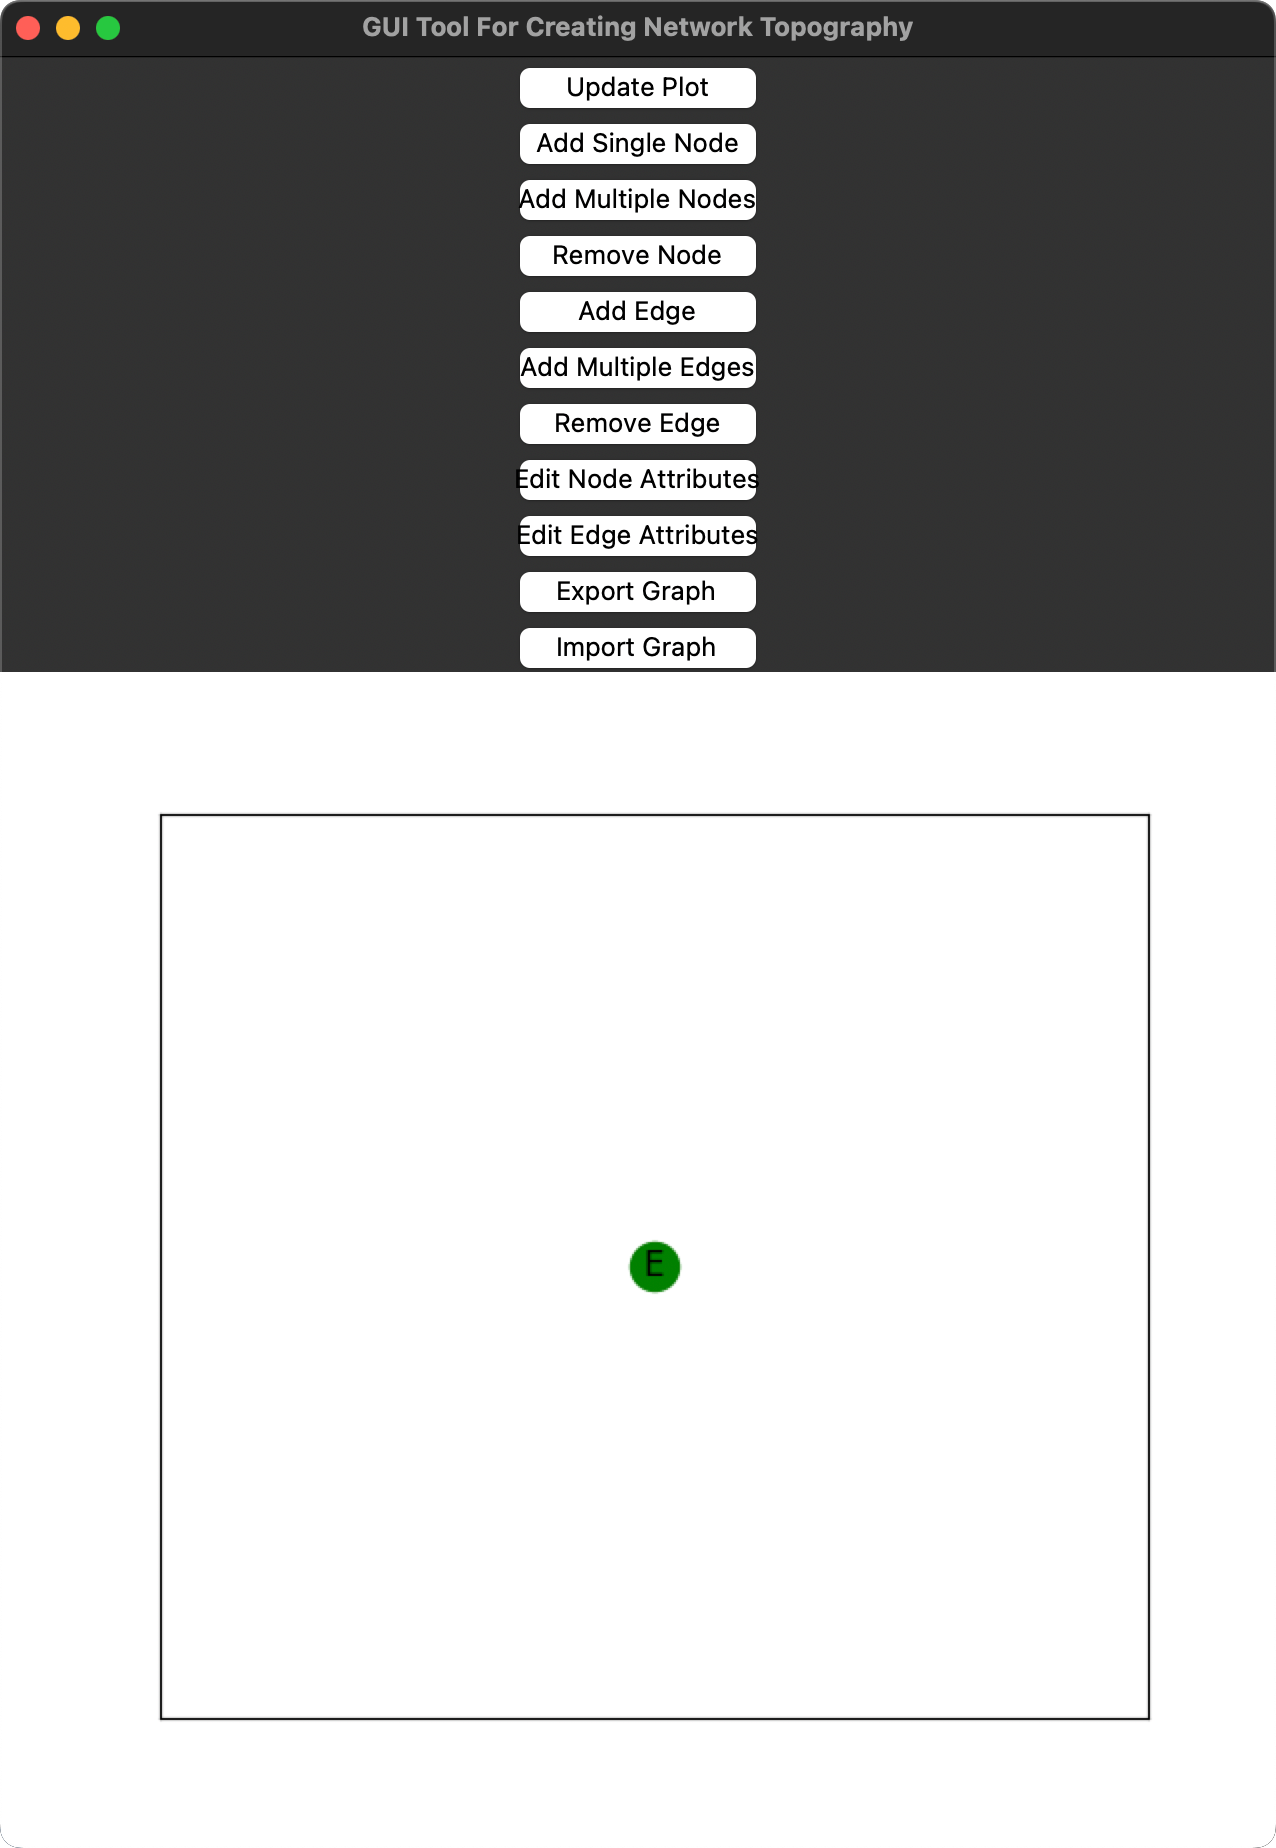
\includegraphics[width=0.5\linewidth]{Screenshots/initial_startup_GUI_tool.png}
    \caption{The GUI tool when you start it up. There are numerous tools that you can use to edit the graph. By default, an environment node holding parameters such as pH and temperature is added. A settings node is added as well, holding settings data to be used for the solver like the type of solver (RK23 or RK45) as well as plotting settings like size of the arrows in the quiver plot. }
    \label{fig:ss:initial_startup_GUI_tool}
\end{figure}
\Cref{fig:ss:initial_startup_GUI_tool} shows the layout of the very simple tool build using tkinter, matplotlib, and networkx %TODO: Citation needed. 
Although the button labels are self-explanatory, the buttons allow the user to add exactly 1 node of either type “P” for phage, “B” for bacteria, or “R” for resource and provide a name. 
That is however tedious for large graphs, so the user can add multiple nodes at the same time. 
The newly created node is provided with default parameter values that the user has to provide beforehand. 
However, if the user forgets this, or doesn't want to, they still able to add, remove, or edit the parameter names and values later. 
The user can remove a node in case of a typo, or they want to change the system. 

The same can be done for the edges, where the edges can either be individually added or removed, or multiple can be created at the same time. 

Finally, the user can import an already saved graph file, or export the graph file to the disk. 


\begin{figure}
    \centering
    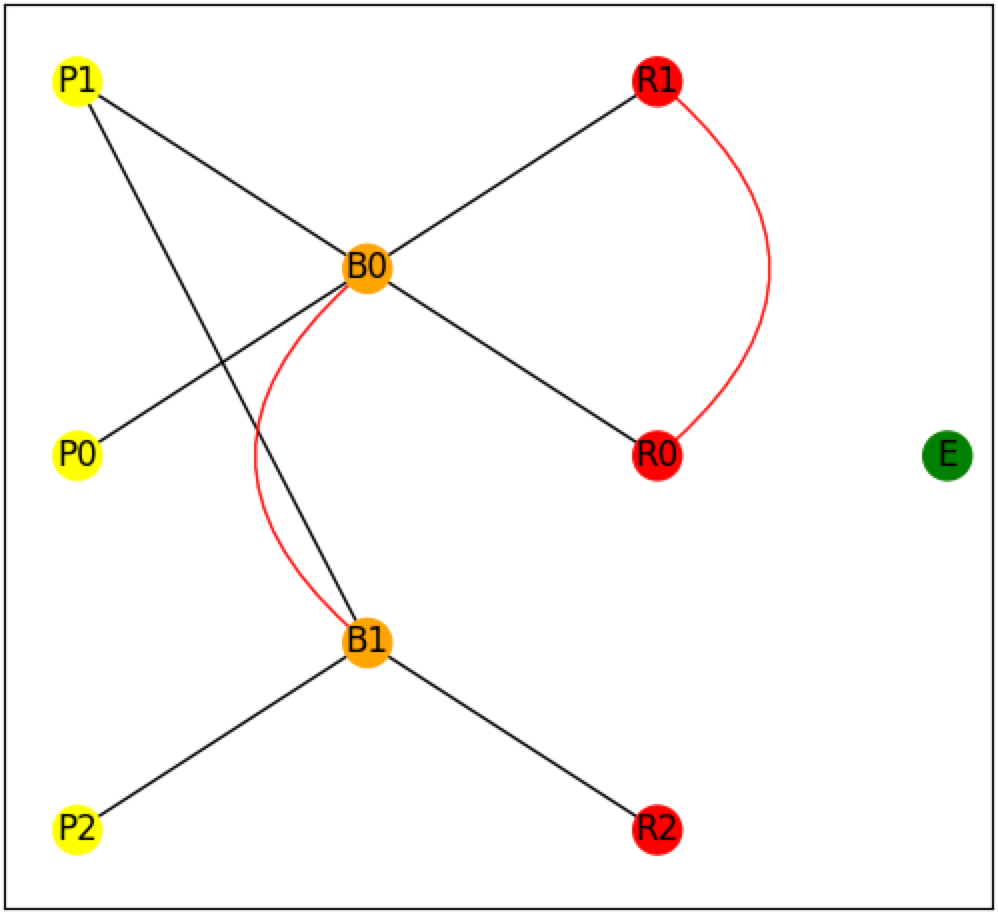
\includegraphics[width=0.5\linewidth]{Screenshots/example_network.png}
    \caption{An arbitrary $3\times2\times3$ network. Phage 0 (P0) interacts/infects bacteria 0 (B0) (and likewise B0 interacts with P0 in some way). P1 infects B0 and B1, etc. Finally, resource 0 (R0) interacts with R1 (an example of this would be a complex sugar degrading into a simple sugar over time). The nature of the interaction needs to be defined and captured in the parameter names, values, and ODE equations. Note: nothing can interact with the environment node.}
    \label{fig:ss:example_network}
\end{figure}
 
Once a network topography capturing the interactions between any number of agents has been created, it would be useful to see how the population count or concentration value changes through time. 
A Python package has been created that allows for uploading a network topography, and with a small script that the user needs to provide, with the setting up of initial parameters and provided equations, runs a numerical solver using SciPy's solve\_ivp() function.  